%\documentclass[11pt, xcolor=dvipsnames,svgnames,x11names]{article}
\documentclass[nohyper,nobib,xcolor=dvipsnames,svgnames,x11names]{tufte-book}

\title{Signals and Systems for Computer Engineers}
\date{Worksheet}
\author[Rahul Bhadani]{Rahul Bhadani}
\publisher{Department of Electrical \& Computer Engineering, The University of Alabama in Huntsville}


%%%%%%%%%%%%%%%%%%%%%%%%%%%%%%%%%%%%%%%%%%
\usepackage{hyperref}
\hypersetup{
    colorlinks=true,
    linkcolor=SeaGreen,
    urlcolor=SeaGreen,
    citecolor=SeaGreen,
    filecolor=SeaGreen
}
\usepackage{amsmath}
\usepackage{amssymb}
\usepackage{xcolor}
\usepackage{tikz}
\usetikzlibrary{backgrounds}
\usetikzlibrary{shadings}
\usepackage{eso-pic}
\usepackage{tkz-euclide}
\usepackage{graphicx}
\usepackage[T1]{fontenc}
\usepackage{wesa}


\newenvironment{multiequation}{%
  \setlength{\abovedisplayskip}{3pt}      % Reduce space above the equation
  \setlength{\belowdisplayskip}{6pt}      % Reduce space below the equation
  \setlength{\abovedisplayshortskip}{3pt} % Reduce space above short equations
  \setlength{\belowdisplayshortskip}{6pt} % Reduce space below short equations
  \begin{equation}%                       % Start an unnumbered equation
    \begin{aligned}%                      % Align multiple lines
}{%
    \end{aligned}%                        % End alignment
  \end{equation}%                         % End equation
}


\definecolor{darkrose}{HTML}{9F3450}
\definecolor{forestgreen}{HTML}{35a17f}
\definecolor{lightindigo}{RGB}{150, 150, 255}
\definecolor{faintred}{RGB}{255, 200, 200}


%%%%%%%%%%%%%%%%%%%%%%%%%%%%%%%%%%%%%%%%%%%
\makeatletter
\renewcommand{\maketitlepage}{%
\begingroup%
\setlength{\parindent}{0pt}

{\fontsize{24}{24}\selectfont\textit{\@author}\par}

\vspace{1.5in}{\fontsize{30}{24}\selectfont\@title\par}


\vspace{0.5in}{\fontsize{20}{14}\selectfont\textsf{\smallcaps{\@date}}\par}




\vfill{\fontsize{14}{14}\selectfont\textit{\@publisher}\par}

\thispagestyle{empty}
\endgroup
}



% Generates the index
\usepackage{makeidx}
\makeindex


\titlecontents{part}%
    [0pt]% distance from left margin
    {\addvspace{0.25\baselineskip}}% above (global formatting of entry)
    {\allcaps{Part~\thecontentslabel}\allcaps}% before w/ label (label = ``Part I'')
    {\allcaps{Part~\thecontentslabel}\allcaps}% before w/o label
    {}% filler and page (leaders and page num)
    [\vspace*{0.5\baselineskip}]% after

\titlecontents{chapter}%
    [4em]% distance from left margin
    {}% above (global formatting of entry)
    {\contentslabel{2em}\textit}% before w/ label (label = ``Chapter 1'')
    {\hspace{0em}\textit}% before w/o label
    {\qquad\thecontentspage}% filler and page (leaders and page num)
    [\vspace*{0.5\baselineskip}]% after
%%%% End additional code by Kevin Godby

\makeatother



\titlecontents{part}%
    [0pt]% distance from left margin
    {\addvspace{0.25\baselineskip}}% above (global formatting of entry)
    {\allcaps{Part~\thecontentslabel}\allcaps}% before w/ label (label = ``Part I'')
    {\allcaps{Part~\thecontentslabel}\allcaps}% before w/o label
    {}% filler and page (leaders and page num)
    [\vspace*{0.5\baselineskip}]% after

\titlecontents{chapter}%
    [4em]% distance from left margin
    {}% above (global formatting of entry)
    {\contentslabel{2em}\textit}% before w/ label (label = ``Chapter 1'')
    {\hspace{0em}\textit}% before w/o label
    {\qquad\thecontentspage}% filler and page (leaders and page num)
    [\vspace*{0.5\baselineskip}]% after
%%%% End additional code by Kevin Godby

\makeatletter
% Redefine chapter to prevent empty pages
\renewcommand{\chapter}{%
  \clearpage% Use clearpage instead of cleardoublepage
  \thispagestyle{plain}%
  \global\@topnum\z@
  \@afterindentfalse
  \secdef\@chapter\@schapter
}

% Alternative approach - modify the openright behavior
\@openrightfalse

% Or if the above doesn't work, try this more direct approach:
\let\cleardoublepage\clearpage
\makeatother



\makeatletter
% Force chapter numbering
\setcounter{secnumdepth}{2}

% Override tufte-book's chapter command to include numbering
\let\oldchapter\chapter
\renewcommand{\chapter}[1]{%
  \refstepcounter{chapter}%
  \oldchapter*{\color{darkrose}{\thechapter. #1}}% Use chapter* with our numbering
  \addcontentsline{toc}{chapter}{\protect\numberline{\thechapter}#1}%
}

% Handle unnumbered chapters (like those created with \chapter*)
\let\oldschapter\@schapter
\renewcommand{\@schapter}[1]{%
  \oldschapter{#1}%
}
\makeatother


% Set table of contents depth to 3 (includes subsubsections)
\setcounter{tocdepth}{3}
\makeatletter
% Chapter entries (level 0) - no indentation
\titlecontents{chapter}%
    [0em]% distance from left margin
    {\addvspace{1em}\bfseries}% above (global formatting of entry)
    {\contentslabel{1.5em}}% before w/ label
    {\hspace{0em}}% before w/o label
    {\titlerule*[.5pc]{.}\contentspage}% filler and page
    [\addvspace{0.5em}]% after

% Section entries (level 1) - slight indentation
\titlecontents{section}%
    [1.5em]% distance from left margin
    {}% above (global formatting of entry)
    {\contentslabel{2.0em}}% before w/ label
    {\hspace{0em}}% before w/o label
    {\titlerule*[.5pc]{.}\contentspage}% filler and page
    []% after

% Subsection entries (level 2) - more indentation
\titlecontents{subsection}%
    [3.5em]% distance from left margin
    {}% above (global formatting of entry)
    {\contentslabel{2.5em}}% before w/ label
    {\hspace{0em}}% before w/o label
    {\titlerule*[.5pc]{.}\contentspage}% filler and page
    []% after

% Subsubsection entries (level 3) - most indentation
\titlecontents{subsubsection}%
    [6em]% distance from left margin
    {}% above (global formatting of entry)
    {\contentslabel{3.0em}}% before w/ label
    {\hspace{0em}}% before w/o label
    {\titlerule*[.5pc]{.}\contentspage}% filler and page
    []% after
\makeatother

% Custom table of contents with 'Content' title that doesn't appear in TOC
\makeatletter
\renewcommand{\tableofcontents}{%
  \clearpage
  \thispagestyle{plain}%
  {\Huge\em Content}\par
  \vspace{1em}
  \@starttoc{toc}%
}
\makeatother

\definecolor{lightorange}{RGB}{255, 245, 230}

% Create a new command for fancy margin notes
\newcommand{\fancymarginnote}[2][0pt]{%
  \marginnote[#1]{%
    \tikz[baseline=(text.base)]{%
      \node[
        fill=lightorange,
        draw=SeaGreen,
        line width=1pt,
        text=darkrose,
        rounded corners=3pt,
        inner sep=4pt,
        text width=\dimexpr\marginparwidth-8pt\relax,
        font=\footnotesize
      ] (text) {#2};
    }%
  }%
}


\begin{document}
\maketitle


\tableofcontents


\chapter{Mathematical Preliminaries}



\section{Complex Numbers}

\begin{enumerate}
    \item \textbf{4pts} Plot the following complex numbers on the complex plane:
    \begin{itemize}
        \item $2+i3$
        \item $3-i2$
        \item $-2-i2$
        \item $-4+j2$
    \end{itemize}


\textbf{Solution:}

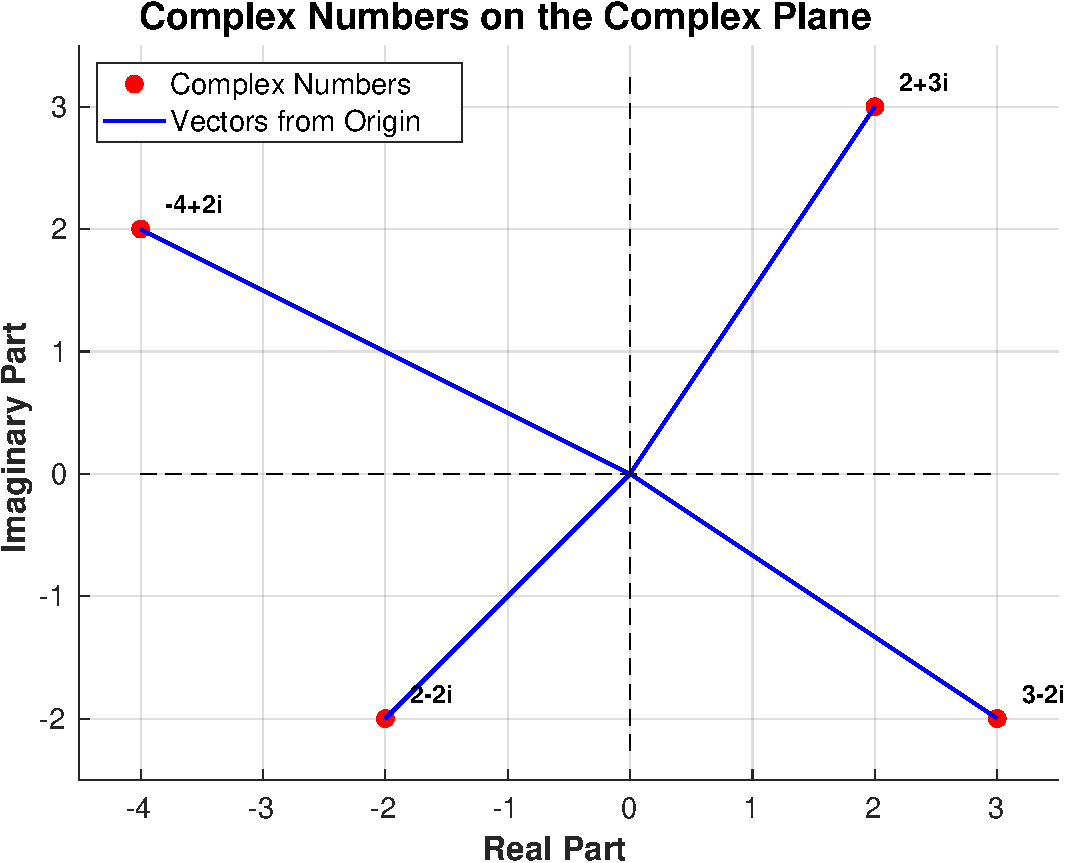
\includegraphics[width=1.0\linewidth]{../Code/figures/Ch01_complex_number_plotting.pdf}


    \item \textbf{4pts} Express $\frac{-1+3i}{2+5i}$ in the form $a+ib$.

\textbf{Solution:}    
    
    \begin{multiequation}
        \frac{-1+3i}{2+5i} &= \frac{-1+3i}{2+5i} \times \frac{2-5i}{2-5i} \\
        &= \frac{-2+5i+6i-15i^2}{2^2+5^2} \\
        &= \frac{-2+11i+15}{4+25} \\
        &= \frac{13+11i}{29} \\
        &= \frac{13}{29} + \frac{11}{29}i
    \end{multiequation}
    

    \item \textbf{2pts} If $Z=3+i5$ is a complex number, what is the value of the modulus $|Z|$?
    
    \textbf{Solution:}
    
    $$|Z| = \sqrt{3^2+5^2} = \sqrt{9+25} = \sqrt{34}$$

    \item \textbf{4pts} Find the roots of the equation $x^2+x+1=0$.

\textbf{Solution:}    
    
    For a quadratic equation $ax^2+bx+c=0$, the roots are given by $x=\frac{-b\pm\sqrt{b^2-4ac}}{2a}$.
    In this case, $a=1$, $b=1$, $c=1$.
    $$x = \frac{-1\pm\sqrt{1^2-4(1)(1)}}{2(1)} = \frac{-1\pm\sqrt{1-4}}{2} = \frac{-1\pm\sqrt{-3}}{2} = \frac{-1\pm i\sqrt{3}}{2}$$

    \item \textbf{2pts} Write the following complex numbers in the polar form:
    \begin{enumerate}
        \item $z=1+i$
        \item $w=\sqrt{3}-i$
    \end{enumerate}
    \textbf{Solution for (a):}
    $|z|=\sqrt{1^2+1^2}=\sqrt{2}$
    $\tan\theta = \frac{1}{1}=1$, so $\theta = \frac{\pi}{4}$.
    In polar form: $z=\sqrt{2}(\cos\frac{\pi}{4}+i\sin\frac{\pi}{4})$.

    \textbf{Solution for (b):}
    $|w|=\sqrt{(\sqrt{3})^2+(-1)^2}=\sqrt{3+1}=\sqrt{4}=2$
    $\tan\theta = \frac{-1}{\sqrt{3}}$, so $\theta = -\frac{\pi}{6}$ (since the number is in the 4th quadrant).
    In polar form: $w=2(\cos(-\frac{\pi}{6})+i\sin(-\frac{\pi}{6}))$.

    \item \textbf{4pts} Find the product of the complex numbers $1+i$ and $\sqrt{3}-i$ in the polar form.
    
    \textbf{Solution:}
    
    From the previous problem, we have:
    $z_1 = 1+i = \sqrt{2}e^{i\pi/4}$
    
    $z_2 = \sqrt{3}-i = 2e^{-i\pi/6}$
    
    $z_1z_2 = (\sqrt{2}e^{i\pi/4})(2e^{-i\pi/6}) = 2\sqrt{2}e^{i(\pi/4-\pi/6)} = 2\sqrt{2}e^{i(\pi/12)}$
    
    In standard polar form: $2\sqrt{2}(\cos\frac{\pi}{12}+i\sin\frac{\pi}{12})$.

    \item \textbf{2pts} Find $(\frac{1}{2}+\frac{1}{2}i)^{10}$.

\textbf{Solution:}    
    
    First, convert to polar form:
    
    $\frac{1}{2}+\frac{1}{2}i = \frac{\sqrt{2}}{2}(\cos\frac{\pi}{4}+i\sin\frac{\pi}{4})$
    
    Using De Moivre's Theorem:
    
    $(\frac{1}{2}+\frac{1}{2}i)^{10} = (\frac{\sqrt{2}}{2})^{10}(\cos(10\cdot\frac{\pi}{4})+i\sin(10\cdot\frac{\pi}{4}))$
    
    $= (\frac{2^{1/2}}{2})^{10}(\cos(\frac{5\pi}{2})+i\sin(\frac{5\pi}{2}))$
    
    $= (\frac{1}{2^{1/2}})^{10}(\cos(\frac{\pi}{2}+2\pi)+i\sin(\frac{\pi}{2}+2\pi))$
    
    $= (\frac{1}{2^5})(0+i\cdot 1) = \frac{i}{32}$

    \item \textbf{2pts} Evaluate or Simplify:
    \begin{enumerate}
        \item $e^{i\pi}$
        \item $e^{-1+i\pi/2}$
    \end{enumerate}
    
    \textbf{Solution for (a):}
    $e^{i\pi} = \cos\pi+i\sin\pi = -1+i(0) = -1$.
    
    \textbf{Solution for (b):}
    $e^{-1+i\pi/2} = e^{-1}e^{i\pi/2} = e^{-1}\bigg( \cos{\tfrac{\pi}{2}} + i \sin{\tfrac{\pi}{2}} \bigg) = \cfrac{1}{e}\bigg(0 + i(1) \bigg)= \cfrac{i}{e}$

    \item \textbf{2pts} Evaluate the expression below and write your answer in the form $a+ib$.
    \begin{enumerate}
        \item $(5-i6)+(3+i2)$
        \item $\frac{3}{4-i3}$
    \end{enumerate}
    \textbf{Solution for (a):}
    $(5-i6)+(3+i2) = (5+3)+(-6+2)i = 8-4i$.
    
    \textbf{Solution for (b):}
    $\frac{3}{4-i3} = \frac{3}{4-i3} \times \frac{4+i3}{4+i3} = \frac{12+i9}{4^2+3^2} = \frac{12+i9}{16+9} = \frac{12+i9}{25} = \frac{12}{25}+\frac{9}{25}i$.

    \item \textbf{2pts} Find the complex conjugate and modulus of the number:
    \begin{enumerate}
        \item $12+i5$
        \item $-1+2\sqrt{2}i$
    \end{enumerate}
    \textbf{Solution for (a):}
    
    Complex conjugate: $12-i5$.
    
    Modulus: $|12+i5| = \sqrt{12^2+5^2} = \sqrt{144+25} = \sqrt{169} = 13$.
    
    \textbf{Solution for (b):}
    
    Complex conjugate: $-1-2\sqrt{2}i$.
    
    Modulus: $|-1+2\sqrt{2}i| = \sqrt{(-1)^2+(2\sqrt{2})^2} = \sqrt{1+8} = \sqrt{9}=3$.

    \item \textbf{2pts} Apply De Moivre's Theorem to simplify:
    \begin{enumerate}
        \item $(1+i)^{20}$
        \item $(1-\sqrt{3}i)^{5}$
        \item $(1-i)^{8}$
    \end{enumerate}

    \textbf{Solution for (a):}
    
    Convert $1+i$ to polar form: $r=\sqrt{1^2+1^2}=\sqrt{2}$, 
    
    $\theta=\tan^{-1}(\frac{1}{1})=\frac{\pi}{4}$.
    
    $1+i = \sqrt{2}(\cos\frac{\pi}{4}+i\sin\frac{\pi}{4})$.
    
    $(1+i)^{20} = (\sqrt{2})^{20}(\cos(20\cdot\frac{\pi}{4})+i\sin(20\cdot\frac{\pi}{4}))$
   
    $= 2^{10}(\cos(5\pi)+i\sin(5\pi)) = 1024(-1+0i) = -1024$.

    \textbf{Solution for (b):}

    Convert $1-\sqrt{3}i$ to polar form: $r=\sqrt{1^2+(-\sqrt{3})^2}=2$, $\theta=\tan^{-1}(\frac{-\sqrt{3}}{1})=-\frac{\pi}{3}$.
    
    $1-\sqrt{3}i = 2(\cos(-\frac{\pi}{3})+i\sin(-\frac{\pi}{3}))$.

    $(1-\sqrt{3}i)^5 = 2^5(\cos(5\cdot(-\frac{\pi}{3}))+i\sin(5\cdot(-\frac{\pi}{3})))$

    $= 32(\cos(-\frac{5\pi}{3})+i\sin(-\frac{5\pi}{3})) = 32(\cos(\frac{\pi}{3})+i\sin(\frac{\pi}{3}))$

    $= 32(\frac{1}{2}+i\frac{\sqrt{3}}{2}) = 16(1+i\sqrt{3})$.

    \textbf{Solution for (c):}
    
    Convert $1-i$ to polar form: $r=\sqrt{1^2+(-1)^2}=\sqrt{2}$, $\theta=\tan^{-1}(\frac{-1}{1})=-\frac{\pi}{4}$.

    $1-i = \sqrt{2}(\cos(-\frac{\pi}{4})+i\sin(-\frac{\pi}{4}))$.

    $(1-i)^8 = (\sqrt{2})^8(\cos(8\cdot(-\frac{\pi}{4}))+i\sin(8\cdot(-\frac{\pi}{4})))$

    $= 2^4(\cos(-2\pi)+i\sin(-2\pi)) = 16(1+0i)=16$.

    \item \textbf{3pts} Use Euler's formula to prove the following formulas for $\cos x$ and $\sin x$:
    \begin{enumerate}
        \item $\cos x = \frac{e^{ix}+e^{-ix}}{2}$
        \item $\sin x = \frac{e^{ix}-e^{-ix}}{2i}$
    \end{enumerate}
    \textbf{Solution:}
    Euler's formula states:
    $e^{ix} = \cos x + i\sin x$
    $e^{-ix} = \cos x - i\sin x$

    To prove (a), add the two equations:
    $e^{ix}+e^{-ix} = (\cos x + i\sin x) + (\cos x - i\sin x) = 2\cos x$.
    Therefore, $\cos x = \frac{e^{ix}+e^{-ix}}{2}$.

    To prove (b), subtract the second equation from the first:
    $e^{ix}-e^{-ix} = (\cos x + i\sin x) - (\cos x - i\sin x) = 2i\sin x$.
    Therefore, $\sin x = \frac{e^{ix}-e^{-ix}}{2i}$.

\end{enumerate}

%---------------------------------------
%---------------------------------------
%---------------------------------------


\section{Trigonometry}
\begin{enumerate}
    \item \textbf{4 pts} Draw a circle and mark $\frac{\pi}{6}$, $\frac{\pi}{3}$, $\frac{\pi}{4}$, and $\frac{3\pi}{4}$.
    
    \textbf{Solution:}
    
    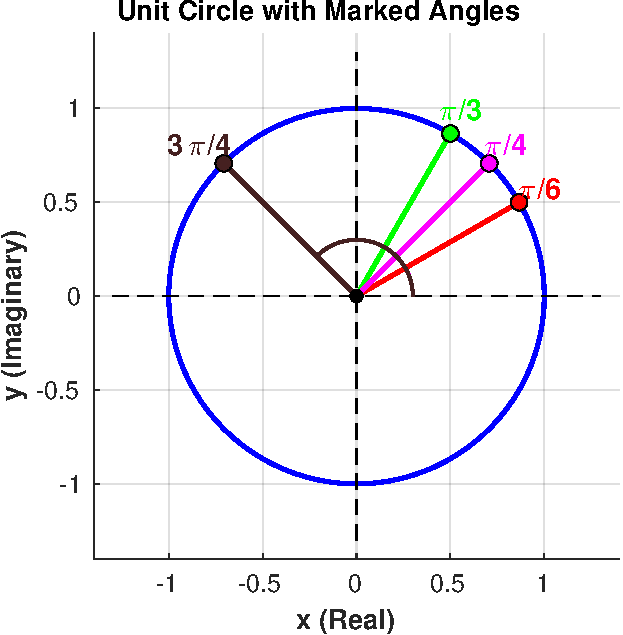
\includegraphics[width=0.6\linewidth]{../Code/figures/Ch01_radian_marking.pdf}

    \item \textbf{1 pts} Convert $\frac{3\pi}{2}$ radians into degrees.
    
     \textbf{Solution:}
     
    \begin{multiequation}
        \frac{3\pi}{2} \times \frac{180^\circ}{\pi} = 270^\circ
    \end{multiequation}

    \item \textbf{3 pts} Find the value of $\theta: 4\sin^2\theta=3$.
    
     \textbf{Solution:}
     
    \begin{multiequation}
        4\sin^2\theta &= 3 \\
        \sin^2\theta &= \frac{3}{4} \\
        \sin\theta &= \pm\frac{\sqrt{3}}{2}
    \end{multiequation}
    
    If $\sin\theta = \frac{\sqrt{3}}{2}$, then $\theta = 60^\circ$ or $\theta = 120^\circ$ (Quadrant I and II).
    
    If $\sin\theta = -\frac{\sqrt{3}}{2}$, then $\theta = 240^\circ$ or $\theta = 300^\circ$ (Quadrant III and IV).


    \item \textbf{3 pts} Find the value of $x: 2\sin^2x-3\sin x+1=0$.
    
     \textbf{Solution:}
     
    \begin{multiequation}
        2\sin^2x-3\sin x+1 &= 0 \\
        2\sin^2x-2\sin x-\sin x+1 &= 0 \\
        2\sin x(\sin x-1)-1(\sin x-1) &= 0 \\
        (2\sin x-1)(\sin x-1) &= 0
    \end{multiequation}
    
    This gives two possible solutions:
    
    $2\sin x - 1 = 0 \implies \sin x = \frac{1}{2}$.
    
    $\sin x - 1 = 0 \implies \sin x = 1$.

    For $\sin x = \frac{1}{2}$, $x = \frac{\pi}{6}$ or $x = \frac{5\pi}{6}$.
    
    For $\sin x = 1$, $x = \frac{\pi}{2}$.
    
    The general solutions are $x = \frac{\pi}{6}+2\pi K$, $x = \frac{5\pi}{6}+2\pi K$, and $x = \frac{\pi}{2}+2\pi K$.

    \item \textbf{5 pts} Prove: $(1-\sin^2(t))(1+\tan^2(t))=1$.
    
    \textbf{Solution:}
    
    \begin{multiequation}
        (1-\sin^2(t))(1+\tan^2(t)) &= (\cos^2(t))(1+\tan^2(t)) \\
        &= \cos^2(t) + \cos^2(t)\tan^2(t) \\
        &= \cos^2(t) + \cos^2(t)\frac{\sin^2(t)}{\cos^2(t)} \\
        &= \cos^2(t) + \sin^2(t) \\
        &= 1
    \end{multiequation}

    \item \textbf{5 pts} Prove: $\frac{\sin^3(t)+\cos^3(t)}{\sin(t)+\cos(t)}=1-\sin(t)\cos(t)$.
    
    \textbf{Solution:}
    
    Using the identity $a^3+b^3=(a+b)(a^2-ab+b^2)$.
    
    Let $a=\sin(t)$ and $b=\cos(t)$.

    \begin{multiequation}
        \frac{\sin^3(t)+\cos^3(t)}{\sin(t)+\cos(t)} &= \frac{(\sin(t)+\cos(t))(\sin^2(t)-\sin(t)\cos(t)+\cos^2(t))}{\sin(t)+\cos(t)} \\
        &= \sin^2(t)+\cos^2(t)-\sin(t)\cos(t) \\
        &= 1-\sin(t)\cos(t)
    \end{multiequation}

    \item \textbf{2 pts} What is the value of $\sin\theta$ and $\cos\theta$ given $\tan\theta=\frac{4}{3}$?
    
    \textbf{Solution:}
    
    $\tan\theta = \frac{4}{3} = \frac{\text{Perpendicular}}{\text{Base}}$.
    
    The hypotenuse is $h = \sqrt{3^2+4^2} = \sqrt{9+16} = \sqrt{25} = 5$.
    
    $\sin\theta = \frac{\text{Perpendicular}}{\text{Hypotenuse}} = \frac{4}{5}$.
    
    $\cos\theta = \frac{\text{Base}}{\text{Hypotenuse}} = \frac{3}{5}$.

    \item \textbf{2 pts} Find the value of $\sin\theta$ and $\cos\theta$ from the triangle.

    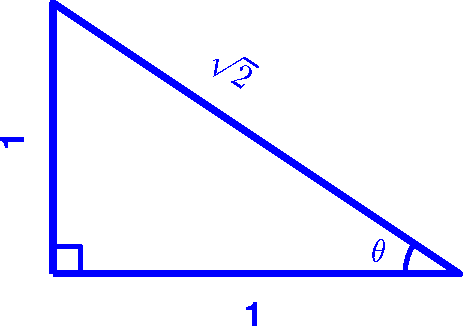
\includegraphics[width=0.4\linewidth]{../Code/figures/Ch01_triangle_drawing.pdf}
    
\textbf{Solution:}

    From the right-angled triangle with sides 1, 1 and hypotenuse $\sqrt{2}$:
    $\sin\theta = \frac{\text{Opposite}}{\text{Hypotenuse}} = \frac{1}{\sqrt{2}}$.
    
    $\cos\theta = \frac{\text{Adjacent}}{\text{Hypotenuse}} = \frac{1}{\sqrt{2}}$.

    \item \textbf{3 pts} Prove $\sin^{-1}(\frac{\sqrt{2}}{2})-\sin^{-1}(\frac{1}{2})=\frac{\pi}{12}$.

\textbf{Solution:}    
    
    $\sin^{-1}(\frac{\sqrt{2}}{2}) = \frac{\pi}{4}$.
    
    $\sin^{-1}(\frac{1}{2}) = \frac{\pi}{6}$.
    
    $\sin^{-1}(\frac{\sqrt{2}}{2})-\sin^{-1}(\frac{1}{2}) = \frac{\pi}{4}-\frac{\pi}{6} = \frac{3\pi-2\pi}{12} = \frac{\pi}{12}$.

    \item \textbf{2 pts} Find the value of $x$ given $2\sin x=1$.
    
    \textbf{Solution:}
    
    $2\sin x=1 \implies \sin x = \frac{1}{2}$.
    
    For $\sin x = \frac{1}{2}$, $x = \frac{\pi}{6}$ or $x = \frac{5\pi}{6}$.

\end{enumerate}

\section{Calculus}

\begin{enumerate}
    \item Using the first principle, differentiate the function $f(x)=e^{2x}$ with respect to $x$.
    
    \textbf{Solution:}
    We are given $f(x)=e^{2x}$. Thus, $f(x+h)=e^{2(x+h)}$.
    The definition of the derivative is $\frac{d}{dx}(f(x))=\lim_{h\to0}\frac{f(x+h)-f(x)}{h}$.
    Substituting the function:
    \begin{multiequation}
        \frac{d}{dx}(e^{2x}) &= \lim_{h\to0}\frac{e^{2(x+h)}-e^{2x}}{h} \\
        &= \lim_{h\to0}\frac{e^{2x}e^{2h}-e^{2x}}{h} \\
        &= \lim_{h\to0}\frac{e^{2x}(e^{2h}-1)}{h} \\
        &= e^{2x} \lim_{h\to0}\frac{e^{2h}-1}{h}
    \end{multiequation}
    We use the known limit $\lim_{x\to0}\frac{e^x-1}{x}=1$.\fancymarginnote{$\lim_{x\to0}\frac{e^x-1}{x}=1$}
    To apply this, we multiply the limit by $\frac{2}{2}$:
    \begin{multiequation}
        &= e^{2x} \left(\lim_{h\to0}\frac{e^{2h}-1}{2h}\right) \times 2 \\
        &= e^{2x} \cdot 1 \cdot 2 \\
        &= 2e^{2x}
    \end{multiequation}
    So, $\frac{d}{dx}(e^{2x})=2e^{2x}$.

    \item If $y=\sin x+e^{x}$, find $\frac{dy}{dx}$.
    
    \textbf{Solution:}
    \begin{multiequation}
        \frac{dy}{dx} &= \frac{d}{dx}(\sin x+e^{x}) \\
        &= \frac{d}{dx}(\sin x)+\frac{d}{dx}(e^{x}) \\
        &= \cos x+e^{x}
    \end{multiequation}

    \item If $y=x^{2}+\sin^{-1}x+\log_{e}x$, find $\frac{dy}{dx}$.
    
    \textbf{Solution:}
    \begin{multiequation}
        \frac{dy}{dx} &= \frac{d}{dx}(x^{2})+\frac{d}{dx}(\sin^{-1}x)+\frac{d}{dx}(\log_{e}x) \\
        &= 2x^{2-1}+\frac{1}{\sqrt{1-x^{2}}}+\frac{1}{x} \\
        &= 2x+\frac{1}{\sqrt{1-x^{2}}}+\frac{1}{x}
    \end{multiequation}

    \item If $y=e^{x}\sin x$, find $\frac{dy}{dx}$. \fancymarginnote{Hint: Use the product rule if $y=u(x)v(x)$, then $\frac{dy}{dx}=\{\frac{d}{dx}u(x)\}v(x)+u(x)\{\frac{d}{dx}v(x)\}$}
    
    \textbf{Solution:}
    Let $u(x)=e^x$ and $v(x)=\sin x$.
    \begin{multiequation}
        \frac{dy}{dx} &= \left(\frac{d}{dx}(e^x)\right)\sin x+e^x\left(\frac{d}{dx}(\sin x)\right) \\
        &= e^x\sin x+e^x\cos x \\
        &= e^x(\sin x+\cos x)
    \end{multiequation}

    \item If $y=\frac{x}{x^{2}+1}$, find $\frac{dy}{dx}$. \fancymarginnote{Hint: Use the quotient rule: $\frac{dy}{dx}=\frac{\{\frac{d}{dx}u(x)\}v(x)-\{\frac{d}{dx}v(x)\}u(x)}{\{v(x)\}^2}$}
    
    \textbf{Solution:}
    Let $u(x)=x$ and $v(x)=x^2+1$.
    \begin{multiequation}
        \frac{dy}{dx} &= \frac{(x^{2}+1)\frac{d}{dx}(x)-x\frac{d}{dx}(x^{2}+1)}{(x^{2}+1)^{2}} \\
        &= \frac{(x^{2}+1)\cdot 1-x\cdot 2x}{(x^{2}+1)^{2}} \\
        &= \frac{x^{2}+1-2x^{2}}{(x^{2}+1)^{2}} \\
        &= \frac{1-x^{2}}{(x^{2}+1)^{2}}
    \end{multiequation}

    \item Evaluate $\int\frac{x+1}{x^{3}+x^{2}-6x}dx$.
    
    \textbf{Solution:}
    First, use partial fraction decomposition:
    \begin{multiequation}
        \frac{x+1}{x^{3}+x^{2}-6x} &= \frac{x+1}{x(x^{2}+x-6)} \\
        &= \frac{x+1}{x(x+3)(x-2)} \\
        &= \frac{A}{x}+\frac{B}{x-2}+\frac{C}{x+3}
    \end{multiequation}
    Setting the numerators equal: $A(x-2)(x+3)+Bx(x+3)+Cx(x-2)=x+1$.
    The coefficients are found to be $A=-1/6$, $B=3/10$, and $C=-2/15$.
    \begin{multiequation}
        \int\frac{x+1}{x^{3}+x^{2}-6x}dx &= \int\left(\frac{-1/6}{x}+\frac{3/10}{x-2}+\frac{-2/15}{x+3}\right)dx \\
        &= -\frac{1}{6}\int\frac{1}{x}dx+\frac{3}{10}\int\frac{1}{x-2}dx-\frac{2}{15}\int\frac{1}{x+3}dx \\
        &= -\frac{1}{6}\ln|x|+\frac{3}{10}\ln|x-2|-\frac{2}{15}\ln|x+3|+C
    \end{multiequation}

    \item Find the indefinite integral of $f(x)=3x^{2}+4x-2$.
    
    \textbf{Solution:}
    \begin{multiequation}
        \int f(x)dx &= \int(3x^{2}+4x-2)dx \\
        &= \int3x^{2}dx+\int4xdx-\int2dx \\
        &= 3\frac{x^{3}}{3}+4\frac{x^{2}}{2}-2x+C \\
        &= x^{3}+2x^{2}-2x+C
    \end{multiequation}

    \item Find $\int x\sin xdx$. \fancymarginnote{Hint: Use integration by parts: $\int u dv=uv-\int v du$}
    
    \textbf{Solution:}
    Let $u=x$ and $dv=\sin xdx$.
    Then $du=dx$ and $v=\int \sin xdx=-\cos x$.
    \begin{multiequation}
        \int x\sin xdx &= x(-\cos x)-\int(-\cos x)dx \\
        &= -x\cos x+\int\cos xdx \\
        &= -x\cos x+\sin x+C
    \end{multiequation}

    \item Solve the differential equation $\frac{dy}{dx}=3x^{2}$.
    
    \textbf{Solution:}

    \begin{multiequation}
        \frac{dy}{dx} &= 3x^{2} \\
        dy &= 3x^{2}dx \\
        \int dy &= \int 3x^{2}dx \\
        y &= \frac{3x^3}{3}+C \\
        y &= x^3+C
    \end{multiequation}
    Thus, the correct answer is $y=x^3+C$.

    \item Solve the equation: $(1+y^{2})y'=\frac{3}{x}$.
    
    \textbf{Solution:}
    Separate the variables:
    \begin{multiequation}
        (1+y^{2})\frac{dy}{dx} &= \frac{3}{x} \\
        (1+y^{2})dy &= \frac{3}{x}dx \\
        \int(1+y^{2})dy &= \int\frac{3}{x}dx \\
        \int 1 dy + \int y^2 dy &= 3\int \frac{1}{x} dx \\
        y+\frac{y^{3}}{3} &= 3\ln|x|+\ln C \\
        y+\frac{y^{3}}{3} &= \ln(C|x|^3) \\
        e^{y+y^{3}/3} &= C|x|^3
    \end{multiequation}

\end{enumerate}

\end{document}

